\chapter{Optimal Control of Two-Level System}
In order to illustrate the use of quantum optimal control it was applied to a two level system with the goal of transferring the initial state $\ket{\psi _0} = \ket{0}_z$ into the target-state $\ket{\psi _{\mathrm{target}}} = \ket{1}_z$. In this model the Hamiltonian in question was
\begin{equation}
	\hat{H} = \Omega \hat{\sigma}_x + u \hat{\sigma}_z \; ,
\end{equation}
where $\sigma_i$'s are Pauli matrices. Thus, the control adjust the rotation around the z-axis in the Bloch sphere representation, while $\Omega$ represents a constant rotational speed around the x-axis giving rise to Rabi oscillations.
For the optimization a steepest descent algorithm was used, such the control was updated at each iteration as
\begin{equation}
	u(t)^{(i+1)} = u(t)^{(i)} - \alpha \nabla \hat{J}(u(t)) \; ,
\end{equation}
where $\alpha$ was found at each iteration using a line search.
In these calculations $\Omega = 1$ was chosen along with the boundary limits of the control $u(0) = 0$ and $u(T) = 2 T$. Furthermore, $\gamma = 0$ was chosen, as the solutions were sufficiently smooth without requiring any penalizing.\\
Note, that for the most direct transfer of the initial state to the target state $u = 0$ would be optimal solution, as $\hat{\sigma}_x$ would rotate the initial state directly into the target state, if no interference from $\hat{\sigma}_z$ is present. However, due to the choice of boundaries of the control, this solution is not viable. Thus, by optimizing the control one is adjusting the rotation around the x-axis, such that $\ket{\psi (T)} = \ket{\psi _{\mathrm{target}}}$, while $u(T) = 2 T$.

\section{Optimization for $T = \frac{\pi}{2}$ } 
An estimate for the QSL of this system can be made using the optimal (but invalid) solution of $u(t) = 0$. Expressing the initial and target state as a linear combination of eigenstates of the $\hat{\sigma}_x$ operator yields
\begin{align}
	\ket{0}_z &= \frac{1}{\sqrt{2}} \left( \ket{1}_x - \ket{0}_x \right) \\ 
	\ket{1}_z &= \frac{1}{\sqrt{2}} \left( \ket{1}_x + \ket{0}_x \right) \; .
\end{align}
Thus, for $\Omega = 1$ and $u(t) = 0$ the Hamiltonian is constant, whereby time evolution can be performed easily
\begin{align}
	\ket{\psi (t)} &= e^{-i \hat{\sigma}_x t} \ket{\psi _0} \nonumber \\
	&= e^{-i \hat{\sigma}_x t } \frac{1}{\sqrt{2}} \left( \ket{1}_x - \ket{0}_x \right) \nonumber \\
	&= \frac{1}{\sqrt{2}} \left( e^{-i t} \ket{1}_x - e^{i t} \ket{0}_x \right) \nonumber \\
	&= e^{-i t} \frac{1}{\sqrt{2}} \left( \ket{1}_x - e^{2 i t} \ket{0}_x \right) \; . \label{eq:timeEvoTwoLevel}
\end{align}
From equation \ref{eq:timeEvoTwoLevel} one sees that $\ket{\psi (T)} = \ket{\psi _{\mathrm{target}}}$ for $T = \frac{\pi}{2}$. Of course in this model $u(t) \neq 0$, however, since $u(T) = \pi$, the rotation around the z-axis for the initial and target state is the same. Thus, it is very likely that $T = \frac{\pi}{2}$ is the QSL of this model.\\

Indeed, performing the optimization for $T = \frac{\pi}{2}$ yields a complete transfer of the initial state into the target state, while $T_1 < T$ fails to converge. Starting with an initial control varying linearly, the optimized control is much different as seen in figure \ref{fig:control}: For the first third of the timespan it remains at zero, which, as described earlier, is the optimal solution when neglecting boundaries. But since it is required that $u(T) = 2 T$, the control first decreases to compensate for the following sharp increase. The resulting path on the Bloch sphere is displayed in figure \ref{fig:path}. Had the control not decreased (resulting in a negative rotation around the z-axis) first, the large upswing in the end would have made the state miss its target.
\begin{figure}[h!]
    \centering
    \begin{subfigure}[t]{0.49\textwidth}
        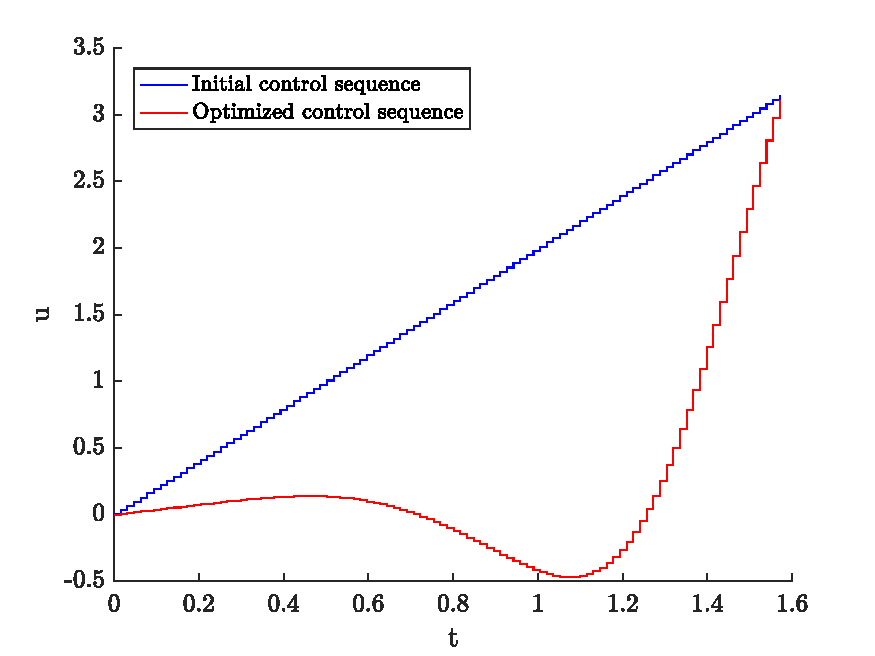
\includegraphics[width=\textwidth]{Figures/control.pdf}
        \caption{\textit{Control, $\boldsymbol{u}(t)$, before and after optimization for $T = \frac{\pi}{2}$.}}
        \label{fig:control}
    \end{subfigure}
    ~
    \begin{subfigure}[t]{0.49\textwidth}
        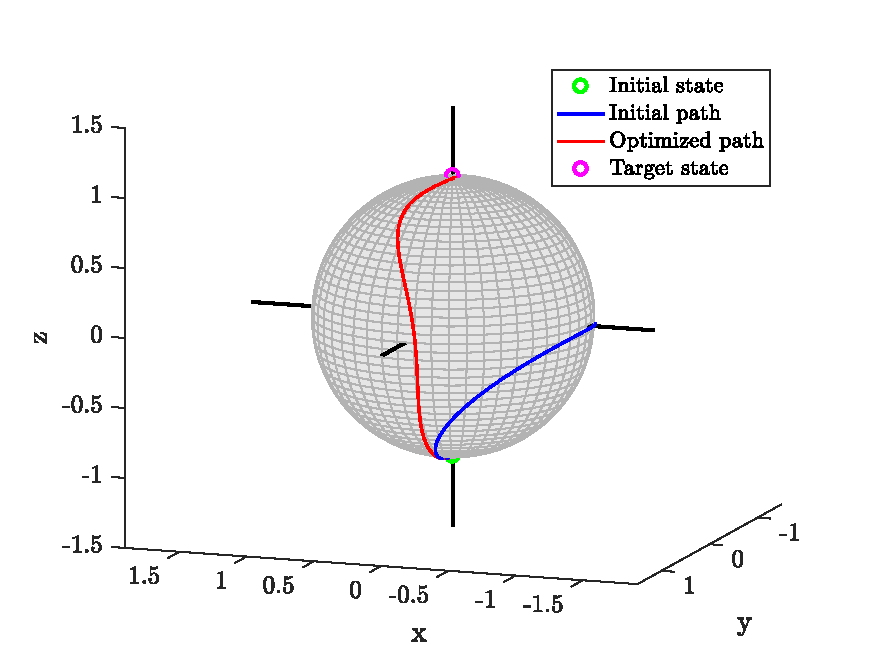
\includegraphics[width=\textwidth]{Figures/path.pdf}
        \caption{\textit{Path traced out by $\psi (t)$ on the Bloch sphere for $T = \frac{\pi}{2}$.}}
        \label{fig:path}
    \end{subfigure}         
	~
    \begin{subfigure}[t]{0.49\textwidth}
        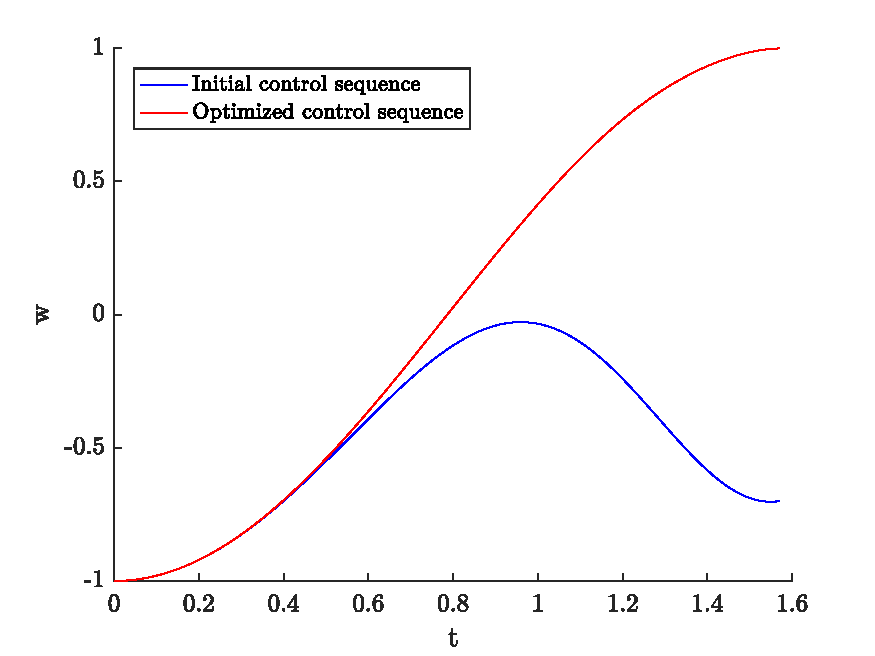
\includegraphics[width=\textwidth]{Figures/pop.pdf}
        \caption{\textit{Population inversion of the system as a function of time for $T = \frac{\pi}{2}$.}}
        \label{fig:population}
    \end{subfigure}
    ~
    \begin{subfigure}[t]{0.49\textwidth}
        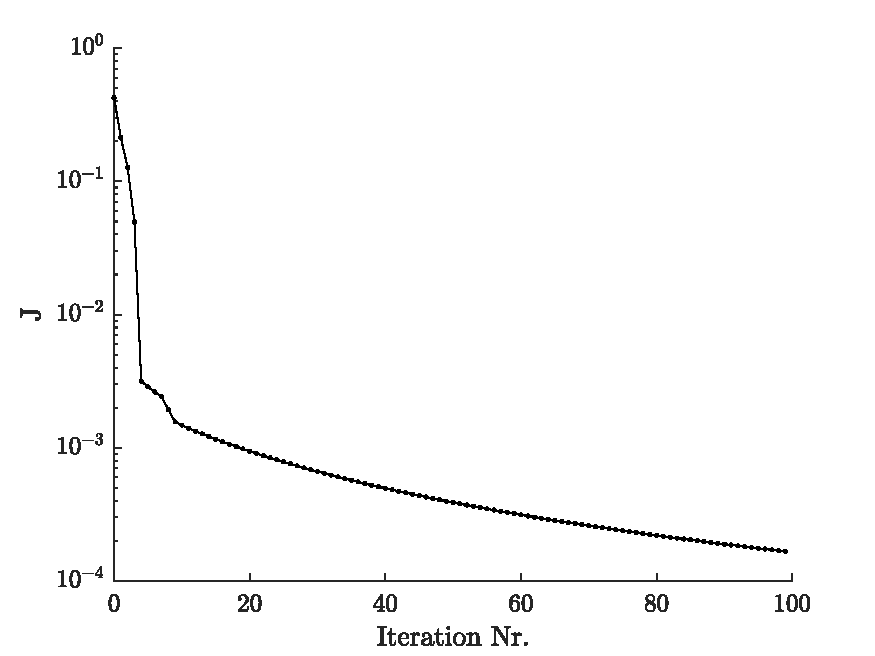
\includegraphics[width=\textwidth]{Figures/cost.pdf}
        \caption{\textit{Reduced cost functional, $\hat{J}$, at each iteration of the optimization for $T = \frac{\pi}{2}$.}}
        \label{fig:cost}
    \end{subfigure}    
\end{figure}
Just how smooth the transfer between the initial and target state is is made clear in figure \ref{fig:population}, where the population inversion, $w = |\braket{1|\psi}|^2 - |\braket{0|\psi}|^2$, is plotted. Although the path on the Bloch sphere is not completely straight, the population inversion is showing the same characteristics as the Rabi oscillations ($|\braket{1|\psi}|^2 \propto \sin \left( \Omega t / 2 \right)$). However, as $T$ is equal to half the period of the Rabi oscillation, the similarity between the solution and Rabi oscillations is to be expected.
Finally, figure \ref{fig:cost} illustrates, how the algorithm finds increasingly better solutions, as the reduced cost functional is gradually decreasing. Since $\gamma = 0$, one can read the fidelity directly of the figure as $F = 1 - 2 J$. Thus, this solution yields a fidelity $F \sim 0.999$, however, since the cost has not yet converged on this figure, an even higher fidelity could be reached with more iterations of the algorithm. 


\section{Optimization for $T = 2$ } 
As described earlier, the GRAPE method will produce a solution, which steers the initial into the target state at $t = T$. Thus, running the algorithm for $T_2 > T_{\mathrm{QSL}}$ should produce a more indirect solution.
This is indeed the case, as seen in figure \ref{fig:control2}, where an Gaussian-like profile has been added on top of the previous solution in order to reach the target state at the desired time. of course this leads to a more indirect path, as illustrated in figure \ref{fig:path2}. Hence, the population inversion of figure \ref{fig:population2} is no longer similar to that of a Rabi oscillation.
\begin{figure}[h!]
    \centering
    \begin{subfigure}[t]{0.49\textwidth}
        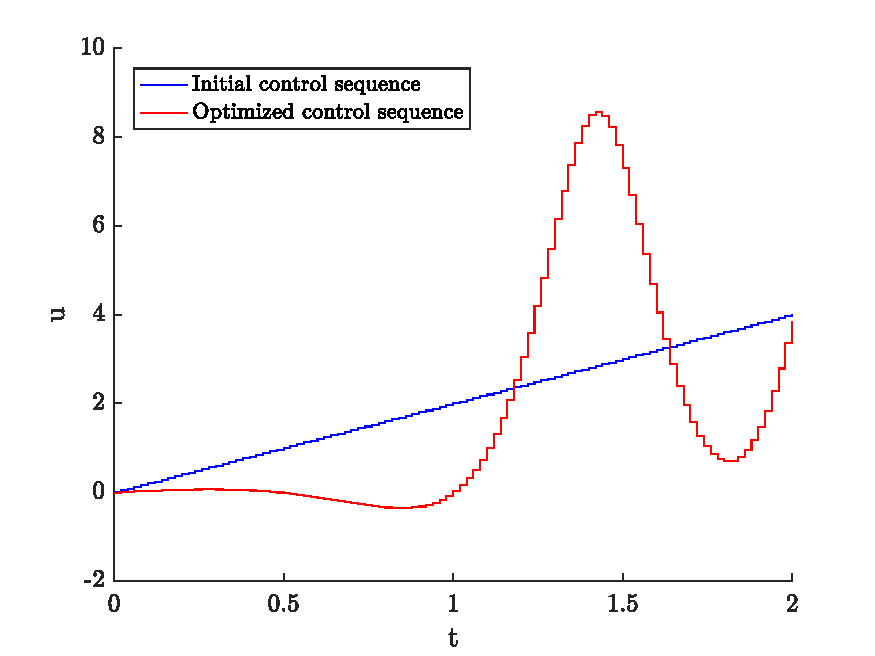
\includegraphics[width=\textwidth]{Figures/control2.pdf}
        \caption{\textit{Control, $\boldsymbol{u}(t)$, before and after optimization for $T = 2$.}}
        \label{fig:control2}
    \end{subfigure}
    ~
    \begin{subfigure}[t]{0.49\textwidth}
        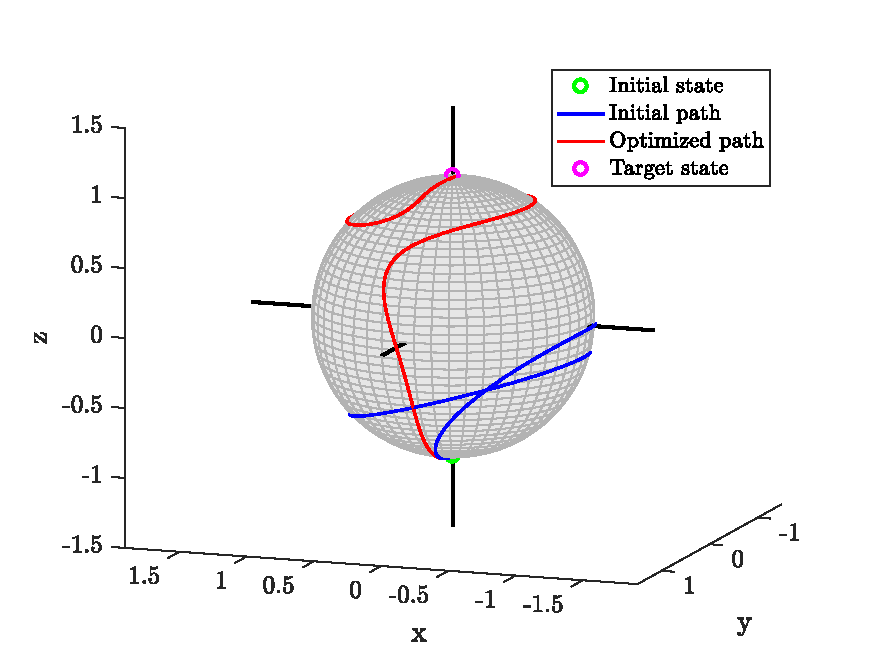
\includegraphics[width=\textwidth]{Figures/path2.pdf}
        \caption{\textit{Path traced out by $\psi (t)$ on the Bloch sphere for $T = 2$.}}
        \label{fig:path2}
    \end{subfigure}   
	~
    \begin{subfigure}[t]{0.49\textwidth}
        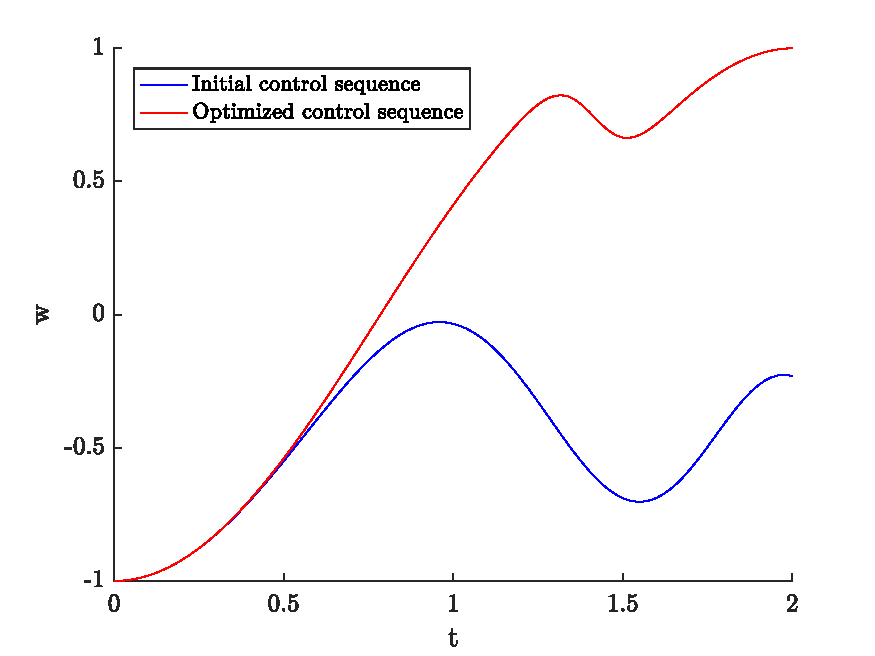
\includegraphics[width=\textwidth]{Figures/pop2.pdf}
        \caption{\textit{Population inversion of the system as a function of time for $T = 2$.}}
        \label{fig:population2}
    \end{subfigure}
    ~
    \begin{subfigure}[t]{0.49\textwidth}
        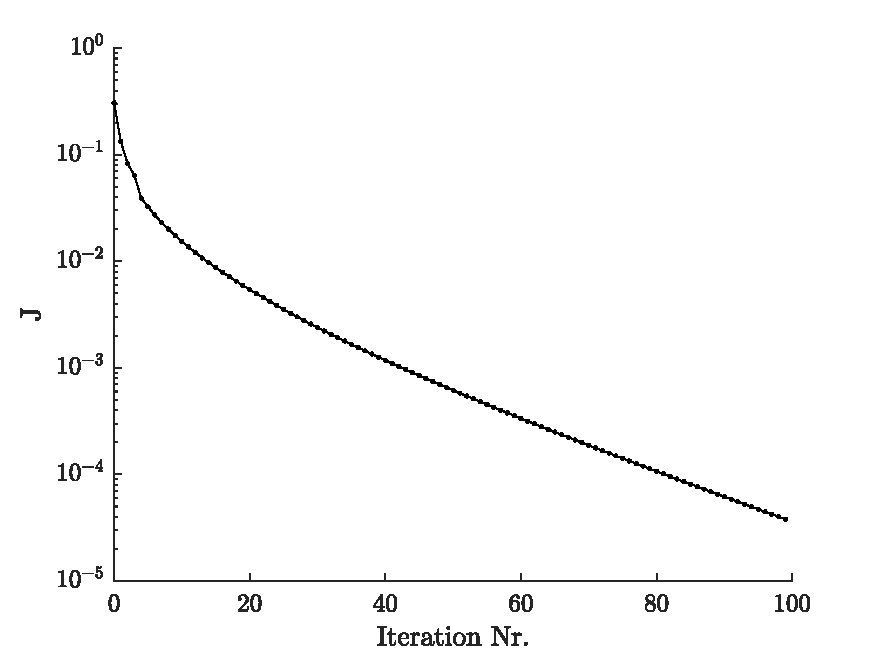
\includegraphics[width=\textwidth]{Figures/cost2.pdf}
        \caption{\textit{Reduced cost functional, $\hat{J}$, at each iteration of the optimization for $T = 2$.}}
        \label{fig:cost2}
    \end{subfigure}     
\end{figure}
Nevertheless, it should be noted that this is a complete valid solution, as it meets all the set requirements.